\documentclass{article}

\usepackage[italian]{babel}
\usepackage[utf8]{inputenc}
\usepackage[export]{adjustbox}
\usepackage{wrapfig}
\usepackage{float}
\usepackage{hyperref}
\usepackage{natbib}
\usepackage[margin=2.0cm]{geometry}
\usepackage{minted}
\usepackage{graphicx}
\usepackage{subcaption}
\usepackage{listings}
\usepackage{color}

\definecolor{dkgreen}{rgb}{0,0.6,0}
\definecolor{gray}{rgb}{0.5,0.5,0.5}
\definecolor{mauve}{rgb}{0.58,0,0.82}
\lstset{frame=tb,
  language=Java,
  aboveskip=3mm,
  belowskip=3mm,
  numbers=left,
  columns=flexible,
  basicstyle={\small\ttfamily},
  numberstyle=\tiny\color{gray},
  keywordstyle=\color{blue},
  commentstyle=\color{dkgreen},
  stringstyle=\color{mauve},
  breaklines=true,
  breakatwhitespace=false,
  tabsize=3
}

\title{%
    \textbf{Laboratorio di sistemi operativi} \\
    Fly-By-Wire}
\author{Gabriele Puliti - \texttt{5300140} - \href{mailto:gabriele.puliti@stud.unifi.it}{\textit{gabriele.puliti@stud.unifi.it}}}
\date{\today}

\begin{document}

\pagenumbering{Roman}
\maketitle

\begin{table}[H]
\begin{tabular}{|c|c|c|}
\hline
\textbf{Elemento Facoltativo}                                                                                                                                                                            & \textbf{Realizzato (SI/NO)} & \textbf{Metodo o file principale} \\ \hline
Utilizzo Makefile per compilazione                                                                                                                                                                       & SI                          & Makefile                          \\ \hline
\begin{tabular}[c]{@{}c@{}}Organizzazione in folder, e creazione dei folder\\ al momento della compilazione\end{tabular}                                                                                 & SI                          & Makefile                          \\ \hline
\begin{tabular}[c]{@{}c@{}}Riavvio di PFC1, PFC2, PFC3 alla \\ ricezione di EMERGENZA\end{tabular}                                                                                                       & No                          & ---                               \\ \hline
\begin{tabular}[c]{@{}c@{}}Utilizzo macro nel Generatore Fallimenti per \\ indicare le probabilità \& PFC Disconnecxt \\ Switch sblocca il processo se bloccato, \\ e lo riavvia altrimenti\end{tabular} & No                          & ---                               \\ \hline
\begin{tabular}[c]{@{}c@{}}PFC Disconnect Switch sblocca il processo \\ se bloccato, e lo riavvia altrimenti.\end{tabular}                                                                               & NO                          & ---                               \\ \hline
\begin{tabular}[c]{@{}c@{}}(continua da sopra) in entrambi i casi, il processo\\  in questione deve riprendere a\\  leggere da punto giusto del file G18.txt\end{tabular}                                & No                          & ---                               \\ \hline
\end{tabular}
\end{table}

\newpage

\pagenumbering{arabic}

\begin{flushleft}

\section{Analisi}

L'obiettivo di questo progetto è quello di costruire una architettura stilizzata, rivisitata e difforme di un sistema chiamato \textbf{Fly-by-wire}. L'obiettivo di questo sistema è quello di andare a sostituire i comandi di un sistema di pilotaggio di un velivolo, tipicamente effattuati da un essere umano, con un sistema digitale. I dati con cui dobbiamo lavorare sono acquisizioni effettuate da un dispositivo mobile chiamato \textbf{GARMIN G18} effettuate in ambiente aperto. Questo dispositivo utilizza un sistema di acquisizione dati, chiamato \texttt{nmea}, che definisce uno standard di rappresentazione del dato grezzo tramite dei record formati da una prima parte, chiamata sentence, e una seconda parte relativa al dato effettivo acquisito. Le sentences sono di diverso tipo, quella che interessa a noi è \textbf{\$GPGLL}. La seconda parte del record varia in base alla sentence, per il problema che a noi interessa risolvere prenderemo in considerazione solo la sentence \$GPGLL a cui corrispondono gli elementi:

\begin{itemize}
    \item Current Latitude
    \item Meridian Direction
    \item Current Longitude
    \item Parallel Direction
    \item Fix taken
    \item Checksum
\end{itemize}

Ognuno di questi elementi è separato da una virgola, un esempio potrebbe essere di questo tipo \textbf{\$GPGLL,4424.8422,N,00852.8469,E,122230,V*3B} estraendo i valori:

\begin{itemize}
    \item \textbf{Current Latitude} = 4424.8422
    \item \textbf{Meridian Direction} = N
    \item \textbf{Current Longitude} = 00852.8469
    \item \textbf{Parallel Direction} = E
    \item \textbf{Fix taken} = 122230
    \item \textbf{Checksum} = V*3B
\end{itemize}

Analizzando un dataset abbastanza grande è possibile ricostruire la traiettoria del dispositivo riuscendo a estrarre istante per istante la velocità istantanea. In una architettura come la nostra la velocità istantanea è una informazione molto importante per comprendere lo stato effettivo del dispositivo.

L'architettura che dobbiamo creare è composta da 5 elementi:

\begin{itemize}
    \item \textbf{PFC}
    \item \textbf{Transducer}
    \item \textbf{Generatore di fallimenti}
    \item \textbf{WES}
    \item \textbf{PFC Disconnect Switch}
\end{itemize}

Ognuno di questi elementi ha una diversa funzionalità e dovrà comunicare con gli altri componenti.

\subsection{PFC}

Questo componente esegue la funzionalità di parsing del dataset e processing del dato acquisito, ogni esecuzione del PFC seguirà questi passi:

\begin{enumerate}
    \item Acquisizione di un nuovo record NMEA GPGLL dal dataset fornito
    \item Estrazione delle coordinate corrispondenti al punto GPGLL
    \item Calcolo della distanza percorsa
    \item Calcolo della velocità istantanea
    \item Invio delle informazioni estratte al Transducer
\end{enumerate}

I PFC nel nostro sistema saranno 3 e comunicheranno con il Transducer usando 3 modalità:

\begin{itemize}
    \item socket
    \item pipe
    \item file
\end{itemize}

\subsection{Transducer}

Questo componente genera per ogni PFC un file di log in cui sarà stampato il valore di velocità calcolato dal PFC corrispondente.

\subsection{Generatore Fallimenti}

Questo dcomponente, chiamato anche FMAN dall'inglese Failure Manager, ad ogni istante seleziona in modo casuale uno dei PFC e con una probabilità indicata nel file di configurazione potrà:

\begin{enumerate}
    \item stoppare il processo
    \item interrompere il processo
    \item far riprendere l'esecuzione di un processo stoppato
    \item alterare il calcolo della velocità
\end{enumerate}

Ogni azione che prenderà sarà salvata in un file di log.

\subsection{WES}

Questo elemento funzionerà da controllore dei PFC e notificatore di malfunzionamenti, istante per istante accederà ai log generati dal Transducer e controllerà se sono i dati sono concordi. Nel caso in cui non fossero concordi possono accadere 2 eventi: un solo PFC è discorde, tutti i PFC sono discordi. Questi eventi vengono notificati al PFC Disconnect Switch che provvederà a gestire i PFC in base alla notificata data. Ogni evento anormale verrà inoltre loggato in un file specifico.  

\subsection{PFCDS}

Questo componente osserva i dati che gli vengono forniti dal WES e in base all'evento reagisce gestendo la risoluzione dei problemi. Se il WES notifica un errore, corrispondente al caso in cui solo 1 PFC è discorde, allora viene controllato se il PFC corrispondente all'errore è ancora in funzione o no e segnalato in un file di log. Se invece viene notificato un segnale di emergenza, corrispondente al caso in cui tutti i PFC sono discordi, allora l'intero sistema viene bloccato.

\section{Sviluppo}

L'intero codice è stato sviluppato e testato su ArcoLinux con compilatore di codice sorgente clang e funzionante anche con gcc. Ho cercato di mantenere una struttura standard per il progetto:

\begin{itemize}
    \item \textbf{src} directory in cui si trova il codice sorgente
    \item \textbf{log} directory in cui vengono generati i logs di esecuzione
    \item \textbf{tmp} generata a runtime in cui sono contenuti i file temporanei usati dai processi
    \item \textbf{bin} directory generata dal Makefile in cui si trovano i binari dei file compilati
    \item \textbf{data} contenente il dataset usato durante lo sviluppo
\end{itemize}

Ho cercato fin da subito di generare un Makefile in modo da rendere comodo il processo di sviluppo riducendo la tediosità dovuta alla compilazione dei nuovi files e generazione dei binari. Ho reso possibile definire il compilatore da usare creando la variabile d'ambiente CC in modo tale da rendere riproducibile il processo di compilazione anche con software differenti dal classico gcc. Ho mantenuto uno standard coerente in tutto il Makefile creando per ogni elemento del codice sorgente una variabile d'ambiente, in questo modo ogni modifica al path del codice sorgente corrisponde una sola modifica nel Makefile, porto sotto un esempio:

\begin{lstlisting}[frame=single]
PREFIX_GLOBAL=src/
PREFIX_PFC=$(PREFIX_GLOBAL)/pfc/
BINDIR=bin/

pfc: utility config 
	@ echo "Compile pfc"
	@ $(CC) -c $(PREFIX_PFC)pfc.c -o $(BINDIR)pfc.o
	@ $(CC) -c $(PREFIX_PFC)structure.c -o $(BINDIR)structure.o
\end{lstlisting}

Gli entries principali che possono essere usati tramite make sono i seguenti:

\begin{itemize}
    \item \textbf{run} Compila l'intero codice e lo esegue (di default il dataset si trova in data/G18.txt)
    \item \textbf{all} Esegue clean e install
    \item \textbf{clean} Elimina le directory temporanee bin, log e tmp
    \item \textbf{install} Compila l'intero codice generando il file eseguibile
\end{itemize}

Il nostro sistema deve gestire 7 processi complessivi: 3 PFC, 1 Transducer, 1 FMAN, 1 WES, 1 PFCDS. Il main, che è possibile trovare su src/main.c, dovrà quindi provvedere all'avvio di questi processi tramite l'utilizzo delle funzioni fork:

\begin{lstlisting}[frame=single]
    pidPFCs[0] = fork();
    if (pidPFCs[0] == 0) {
        pfc(g18Path, PFC_SOCK_SENTENCE, PFC_TRANS_SOCKET);
        exit(EXIT_SUCCESS);
    }
\end{lstlisting}

Nello snippet di codice sopra vediamo la creazione del primo pfc, l'array pidPFCs è l'array che viene usato per raccogliere i pid dei sottoprocessi creati dal main in modo tale da poter usare questi pid nei processi che necessitano di gestire la loro esecuzione, come ad esempio il componente PFCDS. Il main ha solo questa funzione e rimane in attesa della chiusura di questi processi figli, quando tutti saranno conclusi anche il processo padre concluderà. Per evitare la cascata di chiamate wait ho inizializzato una variabile chiamata processCounter con la funzionalità di tenere il conto dei processi attivi in modo tale da risparmiare il conteggio dei processi creati lasciando la responsabilità di questo compito a questo ciclo:

\begin{lstlisting}[frame=single]
    while (processCounter) {
        wait(NULL);
        processCounter -= 1;
    }
\end{lstlisting}

I 3 processi relativi ai PFC sono identici a meno della definizione del tipo di connessione che utilizzano per comunicare con il Transducer, la dichiarazione di questo metodo si trova nell'header src/pfc.h e la sua implementazione in src/pfc.c. Questo metodo funziona principalmente da allocatore di risorse e inoltre inizializza la funzione da chiamare quando il processo riceve un sigusr1, il processing e il reale funzionamento del pfc viene demandato alla funzione chiamata parseNMEA:

\begin{lstlisting}[frame=single]
void parseNMEA(PFC *pPFC, char *sElement, unsigned int connectionType) {
    [...]
}
\end{lstlisting}

La struttura PFC utilizzata come argomento è una delle tante strutture utilizzate dal PFC che vengono usate, per rendere il codice di pfc ho delegato la dichiarazione e gestione di queste strutture a un header esterno che si può trovare sempre nella directory pfc chiamato structure.h e structure.c. Le strutture usate sono queste:

\begin{itemize}
    \item \textbf{PFC} usata per salvare il file path del dataset e il path del log usato per il pfc
    \item \textbf{GLL} dove vengono inseriti i dati estratti da un record nel dataset
    \item \textbf{rawElement} rappresenta il dato grezzo estratto dal dataset
    \item \textbf{PTP} la struttura dati rappresentante un punto della traiettoria del dispositivo, dove vengono inseriti i dati relativi a distanza percorsa e velocità istantanea
\end{itemize}

Queste strutture vengono utilizzate nell'implementazione del parseNMEA, il core di questa funzione si trova nel ciclo while il cui contenuto riporto sotto, eliminando le parti di logging che non hanno responsabilità di processing del dato:

\begin{lstlisting}[frame=single]
    RawElement *pRawElement = malloc(sizeof(RawElement));
    extractRawElements(pRawElement, sLine);
    GLL *pGLL = malloc(sizeof(GLL));
    extractGLL(pGLL, pRawElement);
    addPoint(pPTP, pGLL);
    if (BIAS) {
        pPTP->instantSpeed = (int)round(pPTP->instantSpeed) << 2;
        BIAS = DEFAULT_BIAS;
    }
    char data[64];
    counter += 1;
    sprintf(data, "%i %f", counter, pPTP->instantSpeed);
    sendDataToTrans(pCM, data);
    if (NULL != pPTP->next) {
        pPTP = pPTP->next;
    }
    sleep(CLOCK);
\end{lstlisting}

Questo viene eseguito solo nel caso in cui il record corrisponde ad una sentence GPGLL, quello che fa è:

\begin{enumerate}
    \item estrarre il dato grezzo dal record letto
    \item dal dato grezzo estrarre i dati relativi alle misure GPS
    \item aggiungere questo nuovo punto trovato alla struttura che tiene memoria del percorso fatto
    \item modifica il valore di velocità calcolato nel caso in cui il fman impone un bias sul questo calcolo
    \item invia sia l'identificativo del punto trovato sia la velocità al Transducer e infine dorme per un giro di clock (il clock è modificabile dal file di configurazione config.h, ne parlo successivamente)
\end{enumerate}

Il Transducer, invocato dal main e la cui implementazione si trova sotto la directory src/transducer, elabora questi dati generando per ogni PFC un log speedPFC in cui vengono inseriti i valori del counter del punto estratto e della velocità. Non c'è niente di complesso nell'implementazione di questo componente, possiamo riassumere la sua funzionalità in 3 step: ricezione del dato tramite il canale di comunicazione, stampa del dato su un file di log, dorme 1 giro di clock e ripeti. La struttura che permette la comunicazione tra il PFC e il Transducer è connectionMetadata dichiarata nella libreria utility connection, questa mette a disposizione in maniera trasparente la creazione di server e client in modo semplice e trasparente tramite le funzioni: createSocketClient, createSocketServer, createPipeClient, createPipeServer.

In questo modo ho reso pulito e leggibile il codice che richiedeva la creazione di uno di queste connessioni, con la sola richiesta di dichichiarare una variabile di tipo connectionMetadata in cui sono contenute tutte le informazioni che servono per una di queste due comunicazioni.

Come già detto i processi relativi ai PFC possono essere manipolati dal FMAN che può in ogni momento può inviare uno di questi segnali: SIGTSTOP, SIGINT, SIGCONT e SIGUSR1, il significato di questi segnali è: mettere in pausa, interrompere, riprendere se in pausa e infine eseguire un bias alla misura della velocità. L'implementazione è possibile trovarla nella directory src/fman/, si può notare che per invocare la funzione FMAN è necessario passare la lista dei pid dei PFC perchè solo con questa informazione è possibile osservare un processo che non sia il padre o il processo relativo a FMAN stesso. Considerando che la scelta del processo deve avvenire in modo casuale è necessario utilizzare la funzione rand() della libreria standard stdlib.h, ho implementato due funzioni:

\begin{lstlisting}[frame=single]
double randPercent() {
    time_t seed;
    srand((unsigned) time(&seed));
    return ((double)rand() / (double)RAND_MAX);
}

int randRange(int range) {
    time_t seed;
    srand((unsigned) time(&seed));
    return rand() % range;
}
\end{lstlisting}

La ridefinizione del seed del random è necessaria per non ottenere i soliti valori ogni volta che questa funzione viene chiamata. Per la prima funzione è necessario considerare che il valore rand restituisce un valore tra 0 e RAND\_MAX, quindi prima di restituire un valore di probabilità era necessario normalizzare la distribuzione in modo tale che il valore restituito fosse compreso tra 0 e 1. La seconda restituisce un valore compreso tra 0 e range che viene passato come argomento. Quindi in base al PFC selezionato e alla probabilità estratta vengono azionati i triggher degli eventi sopra descritti utilizzando la chiamata di sistema kill(pid,signal). Gli eventi generati da questo componente modificano il funzionamento dei PFC e di conseguenza i log generati dal Transducer, questi log sono importanti per la coppia di componenti WES e PFCDS che analizzano l'andamento e gestiscono gli errori causati da disallineamenti o malfunzionamenti del sistema. Come FMA il WES, implementato nel sorgente src/wes/, necessita dei pid relativi ai PFC che vengono passati come parametri della funzione wes. Questa funzione in una prima fase si assicura che i file di log siano stati creati con successo, quando i file sono accessibili allora genera la connessione pipe con il PFCDS e inizia l'analisi dei log generati dal Transducer. Il numero del punto acquisito e la velocità sono estratti utilizzando gli stessi metodi usati dai PFC per estrarre i dati grezzi dal record, una volta estratti vengono processati per esaminare se tutti e 3 sono allineati o no, nel caso di disallineamento viene mandato un messaggio al PFCDS formato da: tipo di errore, pid del pfc incriminato. Il messaggio viene generato usando questa porzione di codice:

\begin{lstlisting}[frame=single]
    pidLength = (int)((ceil(log10(pidPFCs[0])) + 1) * sizeof(char));
    data = malloc(1 + strlen(PFCDS_ERROR_SIGNAL) + 1 + pidLength);
    sprintf(data, "%s %d",PFCDS_ERROR_SIGNAL, pidPFCs[0]);
    sendDataToPFCDS(pCM, data);
\end{lstlisting}

La lunghezza del pid viene calcolata in modo dinamico sulla base del numero di cifre, viene poi aggiunta la stringa di errore, configurabile tramite il file config.h, e inviata al PFCDS che deciderà come trattare l'errore. Nel caso di emergenza verrà solo inviato un messaggio senza indicare nessun pid perchè quello che PFCDS dovrà fare è terminare l'esecuzione di tutti i processi, compreso quello del main. L'ultimo componente PFCDS ha la responsabilità di gestire gli errori forniti dal wes, il sorgente è possibile trovarlo in src/pfcds. Nella mia risoluzione ho voluto semplicemente controllare lo stato del PFC incriminato e segnare il suo stato nel file di log relativo al PFCDS senza influire troppo nello stato del PFC stesso, per quanto riguarda invece lo stato di emergenza una volta che viene catturato l'esecuzione di tutti i processi viene terminata. Tutti i dati rilevanti possono essere modificati nel file di configurazione config.h, in questo file è possibile modificare: il nome di tutti i file log, la directory di default del dataset, il valore del clock, le costanti geografiche come il raggio della terra, i nomi dei socket, delle pipe e dei file usati per la comunicazione tra pfc e transducer e infine come richiesto i valori delle probabilità dei triggher di FMAN.

\section{Esecuzione}

Le schermate che inserirò hanno lo stesso formato a 7 riquadri: il riquadro di sinistra corrisponde all'esecuzione del programma, la colonna centrale con 3 riquadri corrisponde ai 3 speedPFC in ordine crescente, nella colonna di destra si ha dall'alto verso il basso: failures.log, status.log e switch.log.

\begin{figure}[H]
\centering
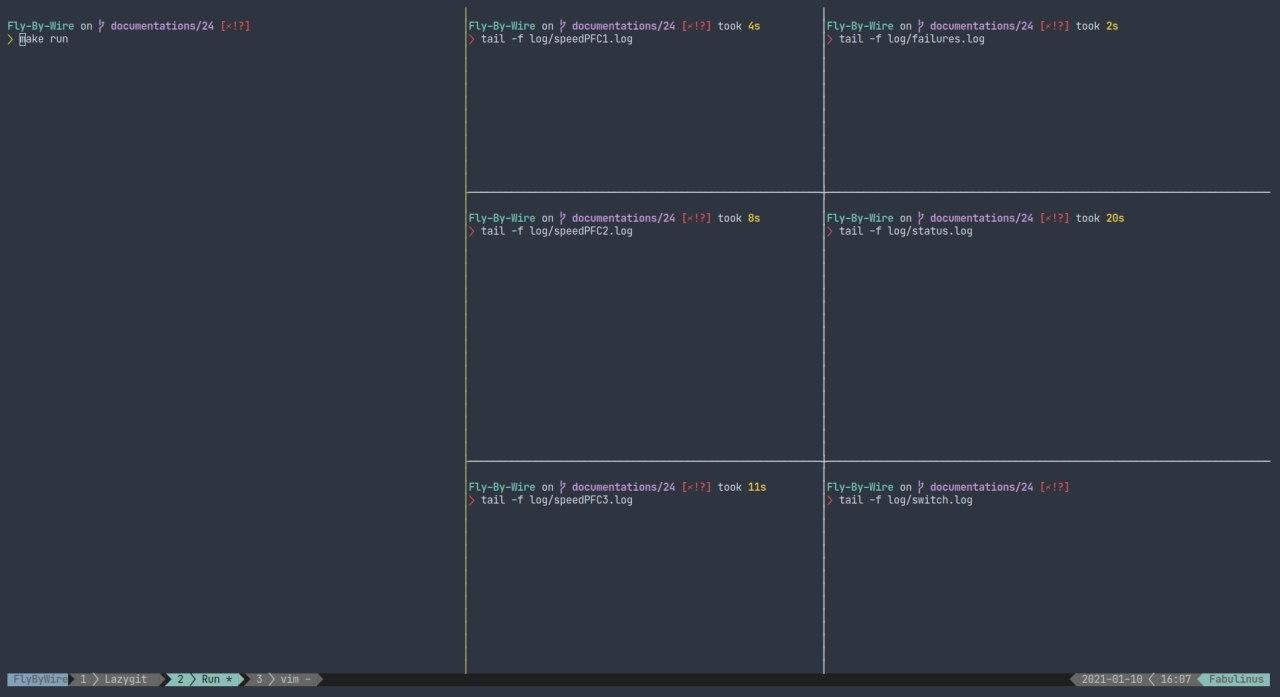
\includegraphics[width=0.8\linewidth]{images/riquadri.jpg}
\end{figure}

L'esecuzione del dataset che abbiamo ho un valore di velocità nullo, quindi rimane fermo per i primi 636 secondi quindi tutti gli speed sono allineati con questo valore a meno di errori fino al counter 636 come si può vedere dall'immagine sotto:

\begin{figure}[H]
\centering
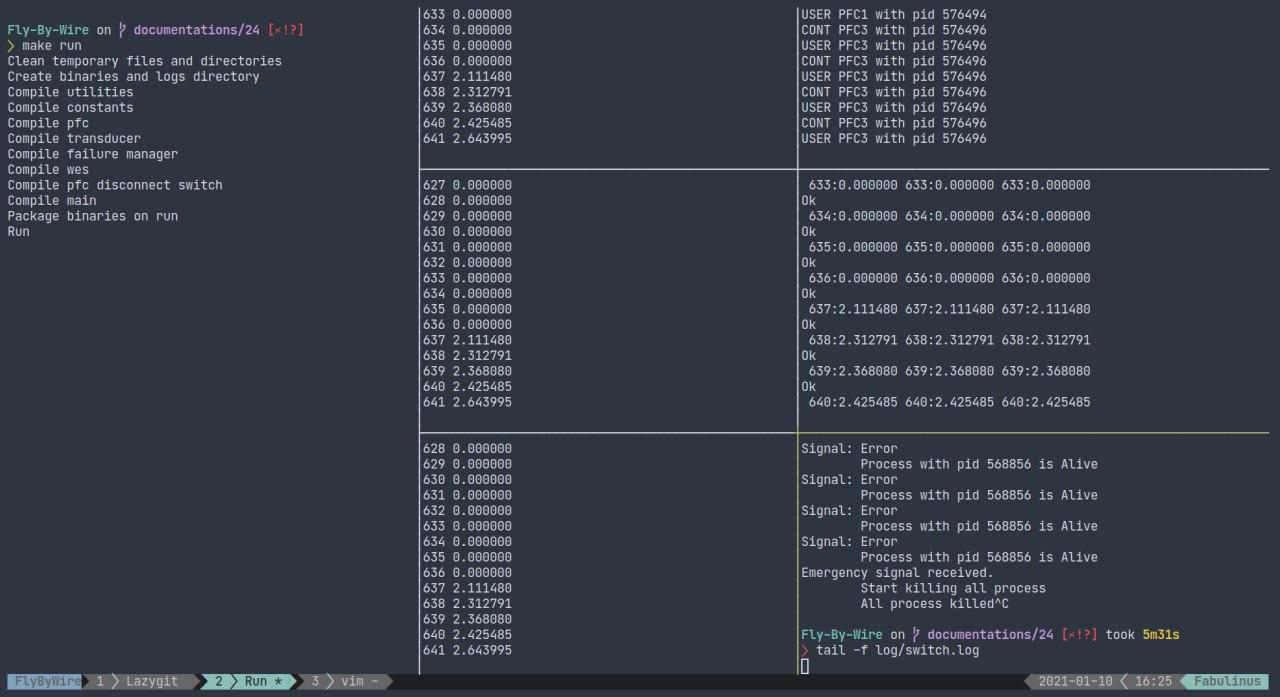
\includegraphics[width=0.8\linewidth]{images/prima.jpg}
\end{figure}

Non appena i PFC si disallineano un segnale di errore viene inviato al pfcds che salva su log questo evento:

\begin{figure}[H]
\centering
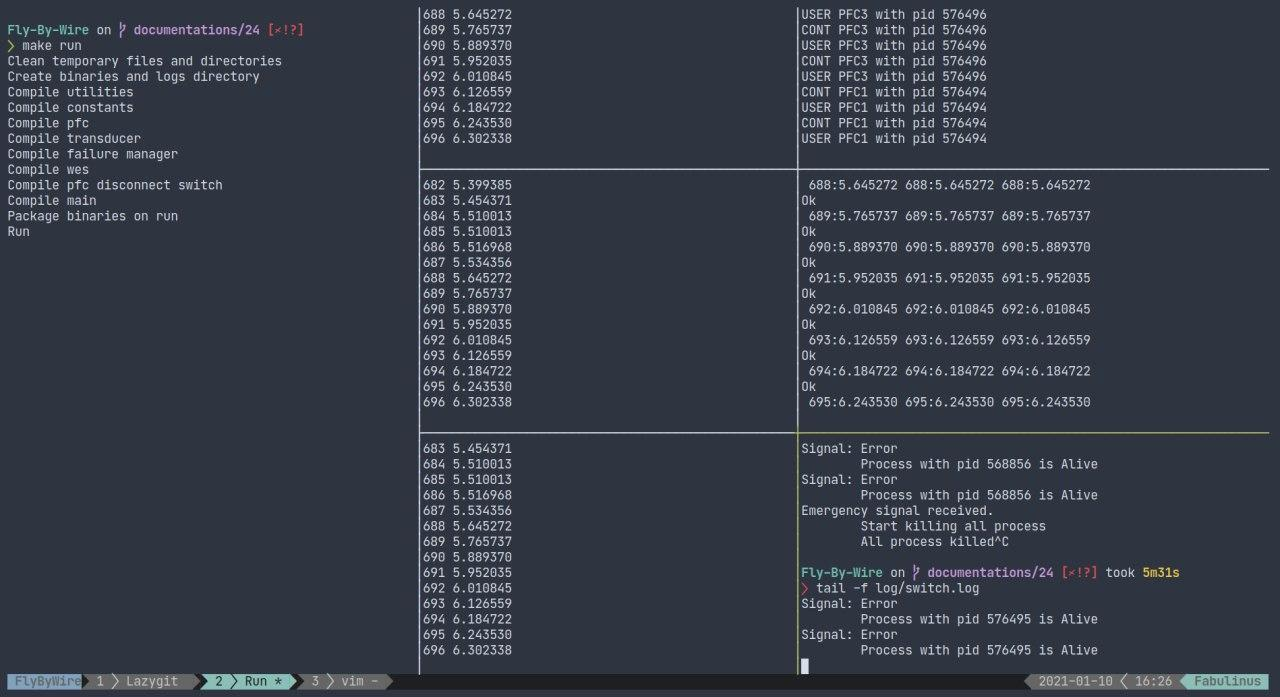
\includegraphics[width=0.8\linewidth]{images/seconda.jpg}
\end{figure}

Al secondo 897 il PFC1 riceve un segnale SIGUSR1 che modifica il suo valore da 31.6 a 128, possiamo notare nei log che il segnale viene correttamente segnalato dal wes come errore:

\begin{figure}[H]
\centering
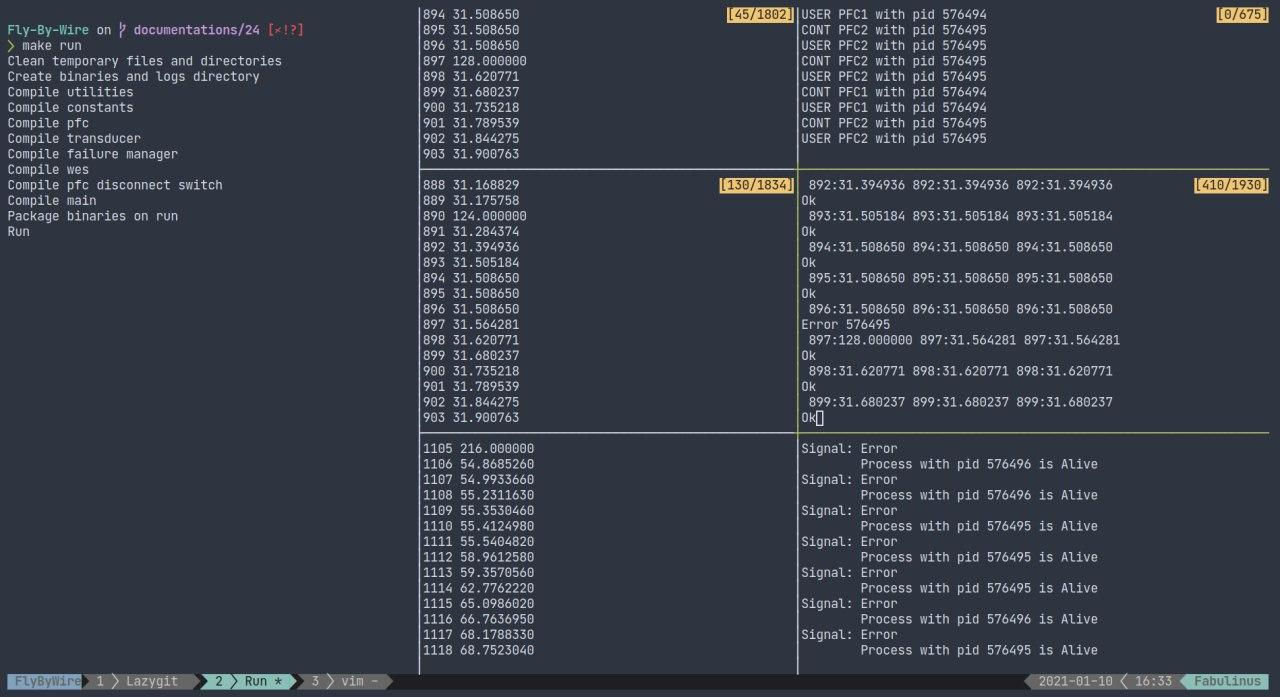
\includegraphics[width=0.8\linewidth]{images/terza.jpg}
\end{figure}

Una volta concluso il processing del dataset tutti i processi si chiudono e come possiamo vedere dal riquadro di sinistra il controllo torna all'utente:

\begin{figure}[H]
\centering
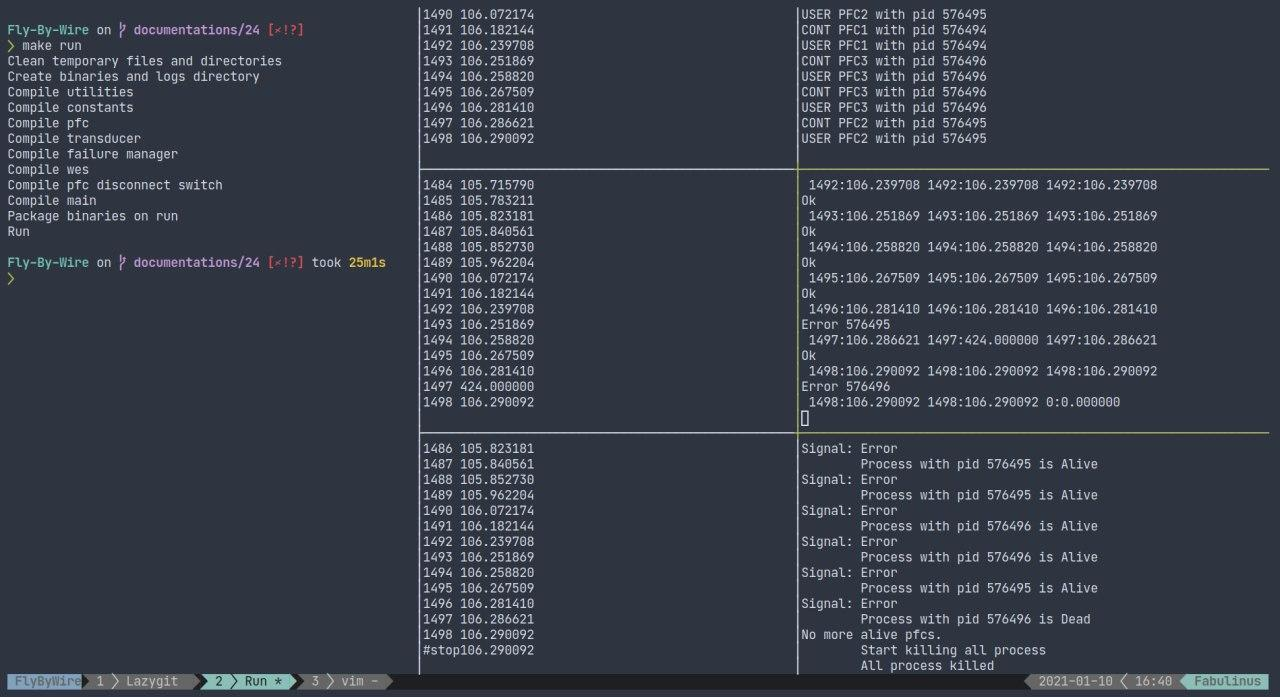
\includegraphics[width=0.8\linewidth]{images/quarta.jpg}
\end{figure}

L'intera lettura del dataset viene letta in 25 minuti. Per completezza porto un esempio di chiusura dovuta a un segnale di emergenza dovuto al disallineamento di tutti e 3 i processi come si può vedere dal riquadro relativo allo status.log:

\begin{figure}[H]
\centering
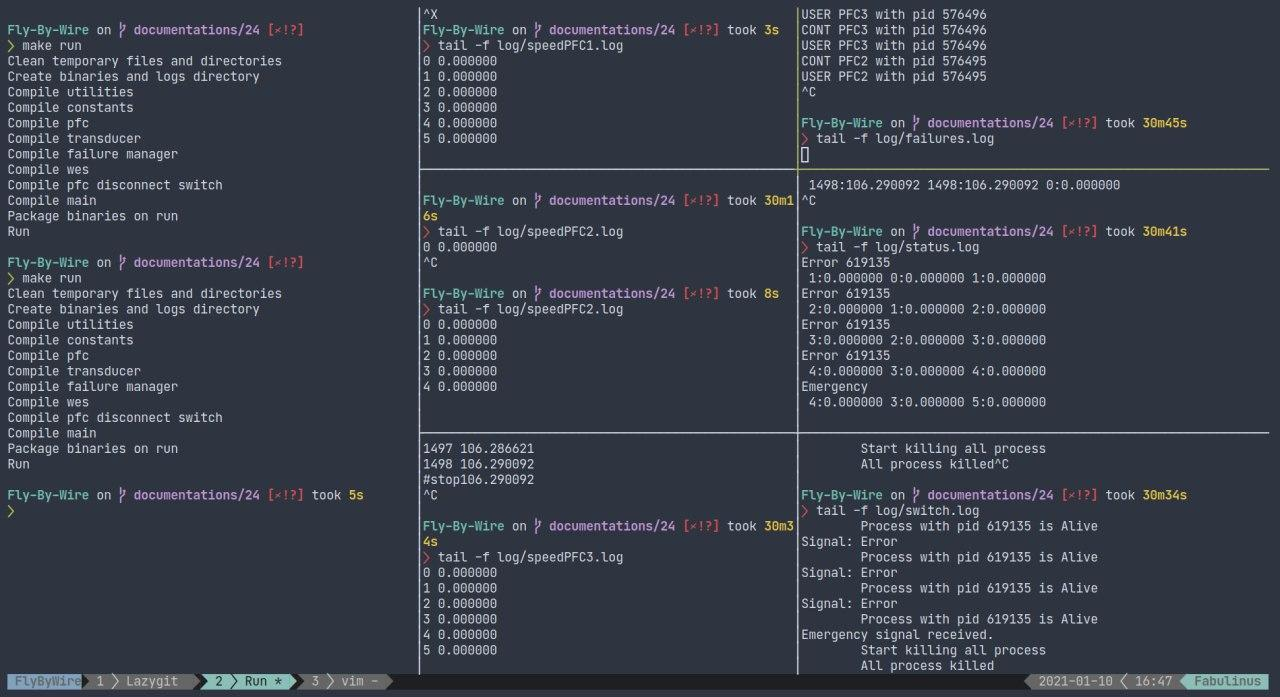
\includegraphics[width=0.8\linewidth]{images/quinta.jpg}
\end{figure}

\section{Conclusioni}

Ci sono alcuni elementi che avrei voluto migliorare come la gestione dei file, per esempio usando la libreria sys/inotify che consente una gestione migliore in termini di risorse, avrei voluto rifattorizzare il codice per renderlo più pulito e performante in termini anche di memoria andandola a liberare quando allocata e non più utilizzata. Il progetto è open source sotto licenza MIT su github all'indirizzo \href{https://github.com/Wabri/Fly-By-Wire}{github.com/Wabri/Fly-By-Wire}, è stato sviluppato utilizzando una metodologia agile rivisitata utilizzando gli strumenti messi a disposizione da github.

\end{flushleft}
\end{document}
